\section{CUDA Implementation}

A Lagrangian simulation naturally lends itself to parallelization, where each thread updates a single particle’s motion. However, a naive implementation of Eq.(\ref{eq:SPH}) would require every thread to iterate over all particles, leading to a $O(n^2)$ complexity per simulation step.

To reduce redundant particle lookups, we adopt the grid-based spatial partitioning method proposed by Green in \cite{green2010particle}. The simulation space is divided into a uniform grid with cell sizes that match the kernel smoothing radius. This allows each particle to determine its grid coordinates and efficiently search only the 26 neighboring cells (8 in 2D).

\begin{figure}[ht!]
    \centering
    \hspace{.2in}
        \subfloat[]{\raisebox{.1\height}{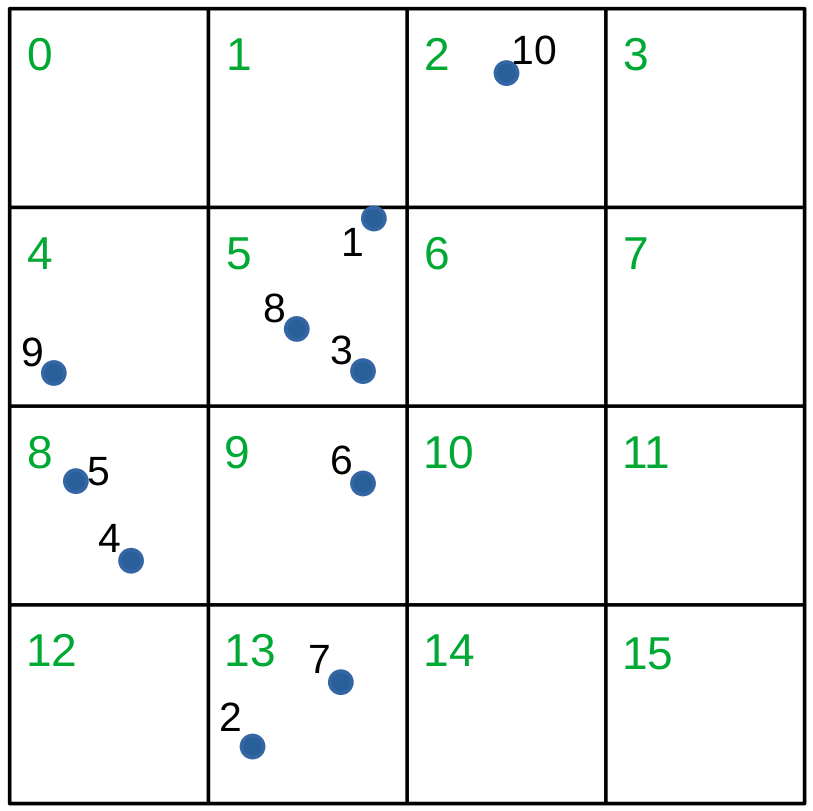
\includegraphics[width=.4\linewidth]{images/part_mapping.png}}}\hspace{.2in}
        \subfloat[]{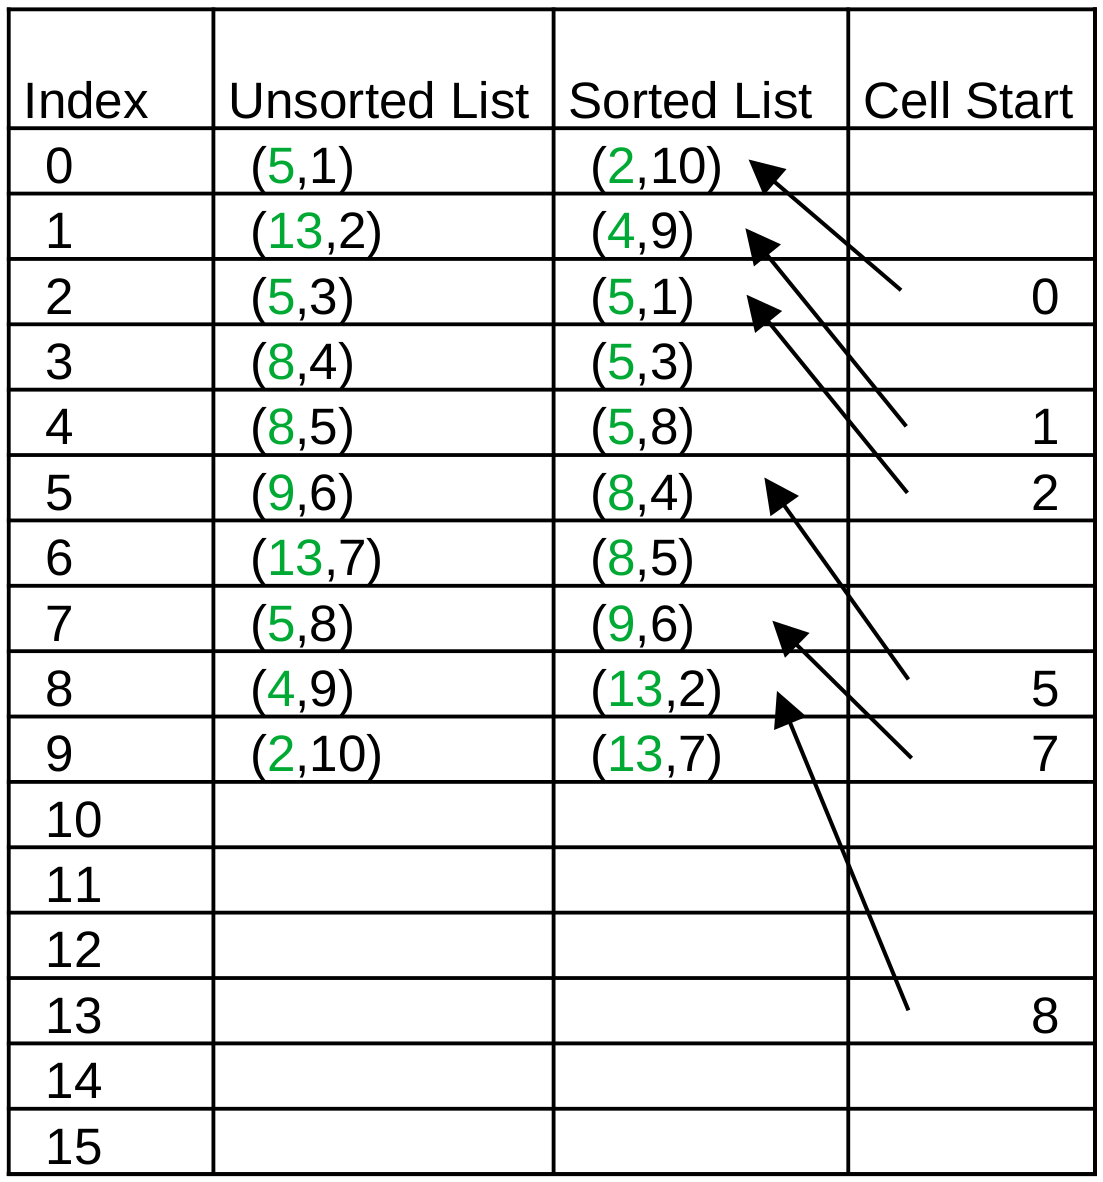
\includegraphics[height=.5\linewidth]{images/part_table.png}}\hspace{.3in}
    \caption{Example of a grid spatial subdivision with the corresponding arrays needed for efficient lookup.}\label{fig:gridPic}
\end{figure}
\noindent
Implementing the grid subdivision requires two additional arrays:
\begin{itemize}
    \item \textbf{Cell-particle array}: which stores, for each particle, a tuple containing the corresponding grid cell ID and the particle ID.
    \item \textbf{Cell start array}: which stores the index (of the cell-particle array) where the $n$-th cell begins. 
\end{itemize}
\noindent
In order for the cell-particle array to be useful it must be sorted using the grid cell ID as the sorting key and, given that we are working with integers, we can efficiently sort it using the Radix sort implementation provided by Nvidia's CUB\footnote{\url{https://nvidia.github.io/cccl/cub/api/structcub_1_1DeviceRadixSort.html}} library.\\
As shown in Figure \ref{fig:gridPic}b, once the cell-particle array is sorted, we can iterate over all particles inside a cell, stopping as soon as the next tuple has a different cell ID.\\

\noindent
Finally, the simulation loop can be summarized as follows:

\begin{algorithm}[H]
\caption{Parallel Fluid simulation}\label{algo:simulation}
$updateGrid()$\\
\ForEach{$p_i \in Particles$ \textbf{parallel}}{
        $\rho_i \gets SPHEstimator(density\_func,\ p_i)$\\
        $f^{pressure}_i \gets SPHEstimator(pressure\_func, \ p_i)$\\
        $f^{viscosity}_i \gets SPHEstimator(viscosity\_func,\ p_i)$\\
        $f^{gravity}_i \gets p_i.velocity.y - 9.81\cdot \rho_i$\\
        $f_i^{total} \gets f^{pressure}_i + f^{viscosity}_i + f^{gravity}_i$\\
        $a_i \gets f_i^{total} / \rho_i$\\
        $v_i \gets p_i.velocity + a_i\cdot\Delta t$\\
        $p_i.position \gets p_i.position + v_i\cdot\Delta t$\\
        $handleCollisions(p_i)$\\
}
\end{algorithm}

\vspace{2mm}
\noindent
Where the functions \texttt{SPHEstimator()} and \texttt{updateGrid()} are the following:
\vspace{2mm}

\begin{algorithm}[H]
\caption{SPHEstimator} \label{algo:sphEstimator}
\SetKwInput{KwInput}{Input}
\KwInput{$(func,\ p_i)$}
$cell\_ID \gets linearGridIndex(p_i) $\\
$qty \gets 0$\\
\ForEach{$nbrCell \in neighbors(cell\_ID)$}{
    \ForEach{$p_j \in nbrCell$}{
        $qty \gets qty + func(p_i,\ p_j)$
    }
}
\Return $qty$
\end{algorithm}

\begin{algorithm}[H]
\caption{updateGrid} \label{algo:GridUpdate}
\ForEach{$p_i \in Particles$ \textbf{parallel}}{
    $cell\_ID \gets linearGridIndex(p_i)$\\
    $GRID[cell\_ID] \gets i$    
}
\end{algorithm}

\noindent
The implementation described in Algorithm \ref{algo:simulation} has two key limitations. First, it involves scattered memory accesses to read all particles within a cell, which causes considerable warp divergence. Second, its efficiency decreases significantly as the number of particles per cell increases, which means that the smoothing radius of the kernel has to be carefully tuned to maintain a good performance level.
\begin{figure}[ht!]
    \centering
    \hspace{.2in}
        \subfloat[]{\raisebox{.07\height}{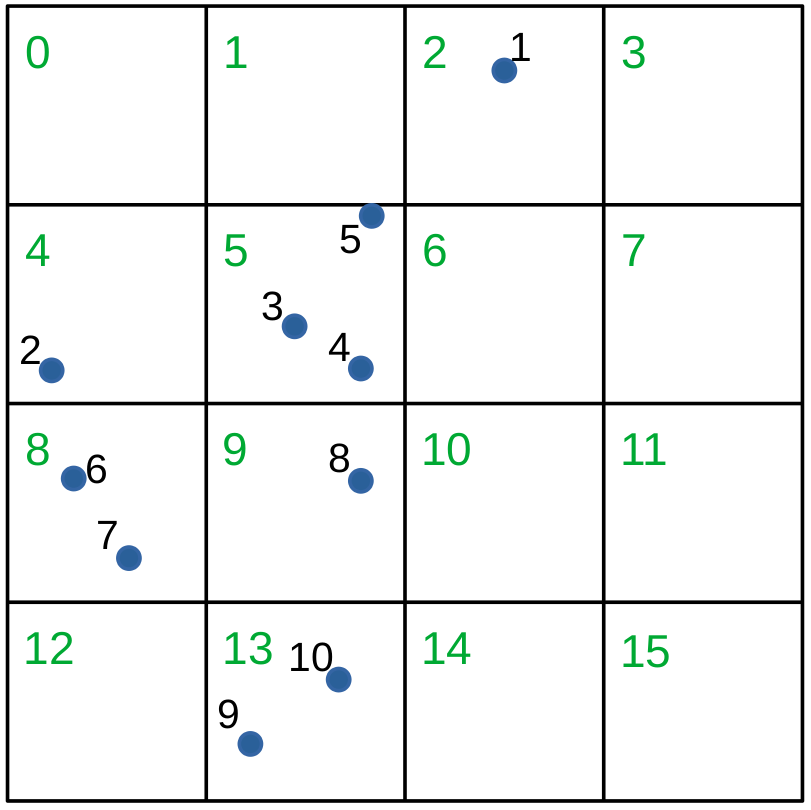
\includegraphics[width=.4\linewidth]{images/part_grid_opt.png}}}\hspace{.2in}
        \subfloat[]{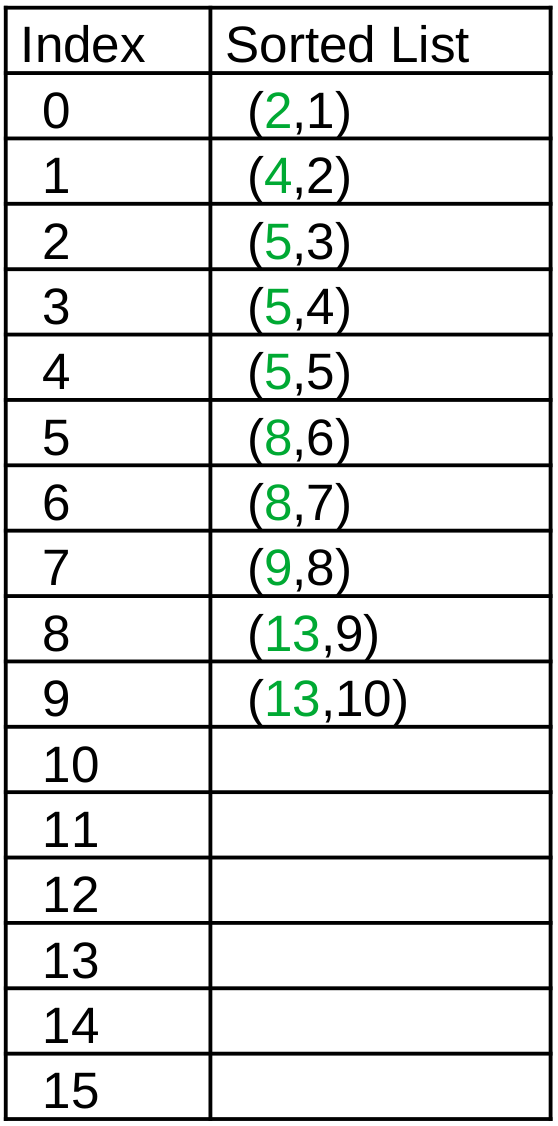
\includegraphics[height=.45\linewidth]{images/part_table_opt.png}}\hspace{.3in}
    \caption{Revised example with particle ID sorting}\label{fig:gridPicOpt}
\end{figure}

\noindent
The first issue can be resolved by sorting the particles according to their positions in the grid, as illustrated in Figure \ref{fig:gridPicOpt}. This approach minimizes warp divergence and improves memory access patterns by enabling coalesced reads and writes while taking advantage of warp broadcasting mechanisms.
This optimization alone, yields a significant speedup, as summarized in Table \ref{tab:perf_comparison} and in Fig. \ref{fig:perf_graphs}
\begin{figure}[ht]
    \centering
    \subfloat{
        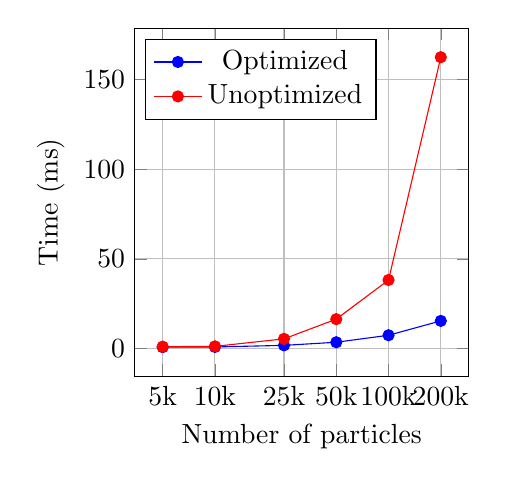
\begin{tikzpicture}
            \begin{axis}[
                xlabel={Number of particles},
                ylabel={Time (ms)},
                xmode=log,
                log basis x={10},
                xtick={5000,10000,25000,50000,100000,200000},
                xticklabels={5k, 10k, 25k, 50k, 100k, 200k},
                legend pos=north west,
                grid=major,
                width=0.48\textwidth,
                height=6cm
            ]
            \addplot[color=blue, mark=*] coordinates {
                (5000, 0.82)
                (10000, 0.92)
                (25000, 1.81)
                (50000, 3.55)
                (100000, 7.45)
                (200000, 15.45)
            };
            \addlegendentry{Optimized}

            \addplot[color=red, mark=*] coordinates {
                (5000, 1.08)
                (10000, 1.26)
                (25000, 5.44)
                (50000, 16.42)
                (100000, 38.26)
                (200000, 162.45)
            };
            \addlegendentry{Unoptimized}
            \end{axis}
        \end{tikzpicture}
    }
    \hfill
    \subfloat{
        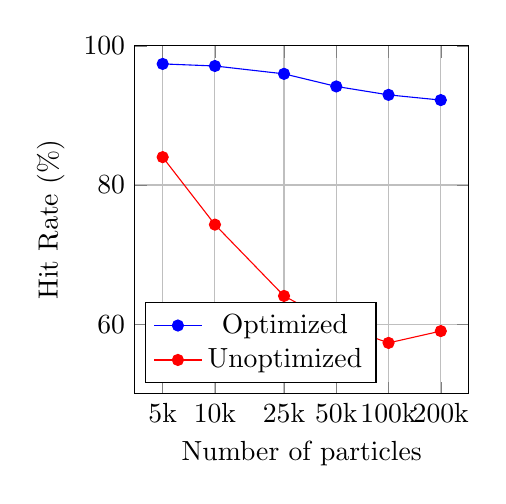
\begin{tikzpicture}
            \begin{axis}[
                xlabel={Number of particles},
                ylabel={Hit Rate (\%)},
                xmode=log,
                log basis x={10},
                xtick={5000,10000,25000,50000,100000,200000},
                xticklabels={5k, 10k, 25k, 50k, 100k, 200k},
                legend pos=south west,
                grid=major,
                width=0.48\textwidth,
                height=6cm,
                ymin=50, ymax=100
            ]
            \addplot[color=blue, mark=*] coordinates {
                (5000, 97.4)
                (10000, 97.1)
                (25000, 95.97)
                (50000, 94.16)
                (100000, 92.95)
                (200000, 92.2)
            };
            \addlegendentry{Optimized}

            \addplot[color=red, mark=*] coordinates {
                (5000, 84.0)
                (10000, 74.3)
                (25000, 64.05)
                (50000, 60.0)
                (100000, 57.3)
                (200000, 59.0)
            };
            \addlegendentry{Unoptimized}
            \end{axis}
        \end{tikzpicture}
    }
    \caption{Optimized vs Unoptimized kernel execution times (left) and L1 cache hit rate (right)}\label{fig:perf_graphs}
\end{figure}


\begin{table}[ht]
\centering
    \begin{adjustbox}{max width=\textwidth}
        \begin{tabular}{@{}lcccccc@{}}
            \toprule
            \texttt{updateParticleKernel} & \textbf{5K} & \textbf{10K} & \textbf{25K} & \textbf{50K} & \textbf{100K} & \textbf{200K} \\
            \midrule
                Execution time (ms)      & 0.82   & 0.92   & 1.81   & 3.55   & 7.45   & 15.45  \\
                Compute throughput (\%)  & 14.50  & 23.05  & 41.80  & 56.50  & 66.41  & 70.10  \\
                L1 Hit rate (\%)         & 97.40  & 97.10  & 95.97  & 94.16  & 92.95  & 92.20  \\
                L2 Hit rate (\%)         & 44.80  & 83.20  & 75.33  & 92.85  & 91.90  & 91.70  \\
                Occupancy (\%)           & 11.50  & 18.80  & 42.70  & 72.40  & 85.42  & 87.49  \\
                Uncoalesced accesses (\%)& 5.00   & 4.00   & 3.00   & 1.00   & 1.00   & 1.00   \\
            \bottomrule
        \end{tabular}
    \end{adjustbox}
\caption{Performance metrics for the optimized kernel with a different number of particles. Measurements taken with a Kernel-function radius of 0.5 units.}\label{tab:perf_comparison}
\end{table}



\begin{figure}[htb!]
    \centering
    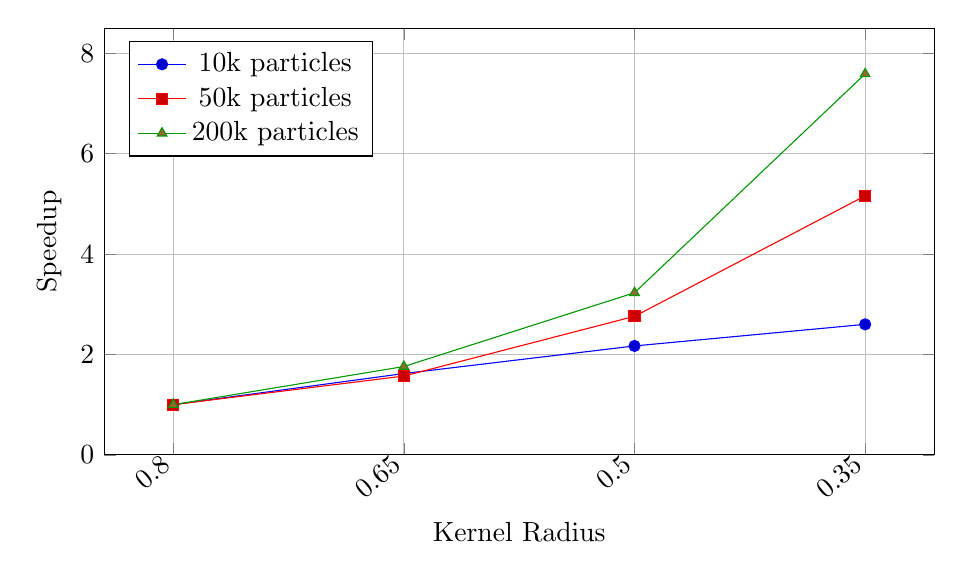
\begin{tikzpicture}
        \begin{axis}[
            xlabel={Kernel Radius},
            ylabel={Speedup},
            xtick={0.8, 0.65, 0.5, 0.35},
            xticklabels={0.8, 0.65, 0.5, 0.35},
            x tick label style={rotate=40, anchor=east},
            x dir=reverse,
            ymin=0,
            ymax=8.5,
            width=\textwidth,
            height=7cm,
            legend pos=north west,
            mark options={solid},
            grid=major
        ]
        \addplot+[blue, mark=*] coordinates {
            (0.8, 1.00)
            (0.65, 1.62)
            (0.5, 2.17)
            (0.35, 2.60)
        };
        \addlegendentry{10k particles}

        \addplot+[red, mark=square*] coordinates {
            (0.8, 1.00)
            (0.65, 1.57)
            (0.5, 2.76)
            (0.35, 5.16)
        };
        \addlegendentry{50k particles}

        \addplot+[green!60!black, mark=triangle*] coordinates {
            (0.8, 1.00)
            (0.65, 1.76)
            (0.5, 3.23)
            (0.35, 7.59)
        };
        \addlegendentry{200k particles}
        \end{axis}
    \end{tikzpicture}
    \caption{Speedup of kernel execution time for various SPH kernel radii.}\label{fig:radius_speedup}
\end{figure}

\noindent
Finally, the latter limitation can be addressed by tuning the kernel smoothing radius, in order to reduce the number of particles per grid cell, as shown in Fig.\ref{fig:radius_speedup}. Unfortunately, reducing the kernel radius too much increases the instability of the simulation. Such instability is also inversely proportional to the temporal resolution of the simulation, thus, in order to be used in a real-time application with a timestep of 1/60th of a second, the radius should be kept above 0.5 units.